
\section{Introduction}

{
    Ant colonies offer an interesting view of collective behavior. 
    The ability to track multiple objects within these colonies is essential for understanding their behavior and has beneficial implications for biology research.
}

{
    This project explores various approaches within the \textbf{tracking by detection} methodology, 
    evaluating \textbf{deep learning-based detection} models for precise and efficient \textbf{multiple object tracking}. 
    Ants, with their complex movements and unique social structures within colonies, provide an ideal subject for this research.
}

{
    Recognizing the profound impact that tracking technology can have on biological investigations, 
    this project collaborates closely with the Ecología Teórica y Computacional group from the \ac{CEAB} within the \ac{CSIC}. 
    This group from the \ac{CSIC}, an institution in the field of scientific research, has provided essential unlabeled data that forms the foundation of our research.
}

{
    Beyond the development of a multiple object tracking software tailored to the \ac{CSIC}'s environment, 
    this project also provides the essential software for training for each element of the tracker and a user-friendly tutorial for annotating new training videos, 
    leveraging the power of automatic tracking results.
}

{
    As we delve into this thesis, we will examine the intricacies of the chosen tracking methodology including ants small size, high visual similarity, and occasional non-linear motion. 
    The accompanying block diagram (Figure \ref{fig:block_diagram} within the methodology section) illustrates our approach. 
    Through this dedicated work, we aim to deepen the understanding of ant behavior, offering valuable contributions to the realm of animal behavior studies.
}

\clearpage

\needspace{0.25\textheight}
\subsection{Work plan}

{
    The tracking by detection problem is divided into four critical components: 
    \textbf{detection}, \textbf{estimation}, \textbf{association}, and \textbf{track management}, offering a comprehensive solution.
}

{
    The research plan contains a set of five core objectives, each contributing to the goal of this project, 
    guiding our exploration of multiple object tracking using the tracking by detection methodology:
}

\begin{itemize}
    \item {
        \textbf{Location Model (Association Component)}:  
        This objective focuses on the application of a location model based on estimations and matchings. 
        The research emphasis lies on the development of position estimators and position matching metrics and algorithms.
        The performance can be enhanced by the implementation of expert knowledge and heuristics specifically tailored to the ant tracking problem. 
        }
    \item {
        \textbf{Appearance Model (Association Component)}: 
        This objective focuses on the training of an appearance description model for capturing distinctive visual features to distinguish individual ants.
    }
    \item {
        \textbf{Detection Model}: 
        The successful localization of ants with accuracy and efficiency is reliant on a robust detection model. 
        This objective encompasses the training of an advanced object detection model, a critical component of our tracking system.
    }
    \item {
        \textbf{Postprocessing}: 
        This step explores the refinement of the tracking results. 
        It involves exploring various techniques, including path matching models, the application of appearance descriptors on sequences, and track interpolation.
        }
    \item {
        \textbf{Datasets Annotation}: 
        We aim to significantly reduce the time required for annotating datasets. 
        This step is fundamental for enhancing dataset readiness and expediting the tracking process.
        }
\end{itemize}

\paragraph{Data Availability Challenges}

{
    Throughout the project, we encountered various phases of data availability; each one with a different setting. 
    These phases of data availability were pivotal in shaping our research: 
}

\begin{enumerate}
    \item The first phase mainly facilitated the analysis of location models.
    \item The second phase allowed the training for both the appearance and detection models.
    \item The third phase was mainly used for testing and evaluation.
\end{enumerate}

\paragraph{Deviations from Initial Plan}

{
    These data challenges demanded adaptations to our research plan. 
    The scarcity of labeled data postponed the path matching model training; 
    at the end, it was discarded as a potential future task. 
    Furthermore, the implementation of expert knowledge was impossible 
    because the experts need this project to obtain that knowledge; 
    at the end of their research, it could be implemented to validate their results.
}


%
%\begin{figure}[!p]
%    \centering
%    \begin{subfigure}[b]{0.8\linewidth}
%        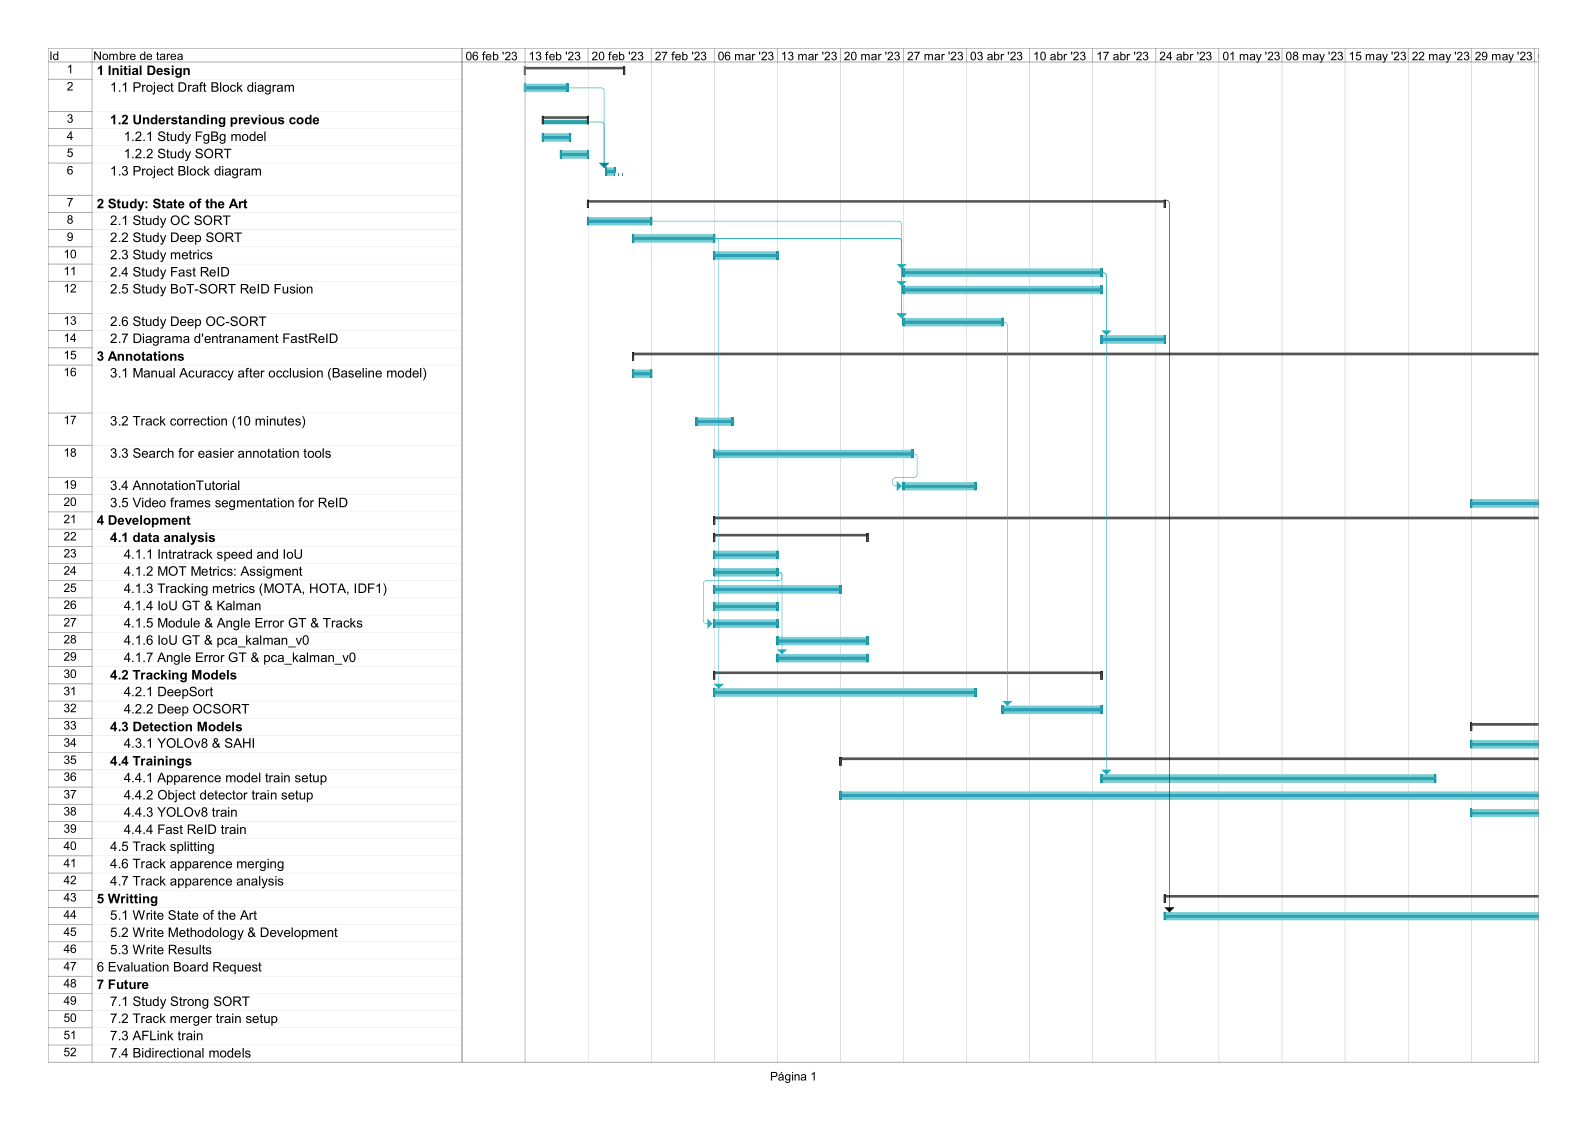
\includegraphics[width=\linewidth]{figures/03_introduction/gantt1.png}
%        \caption[Project's Gantt diagram 1]{\footnotesize{Gantt diagram of the first half of the project}}
%        \label{fig:gantt_1}
%    \end{subfigure}
%    \begin{subfigure}[b]{0.8\linewidth}
%        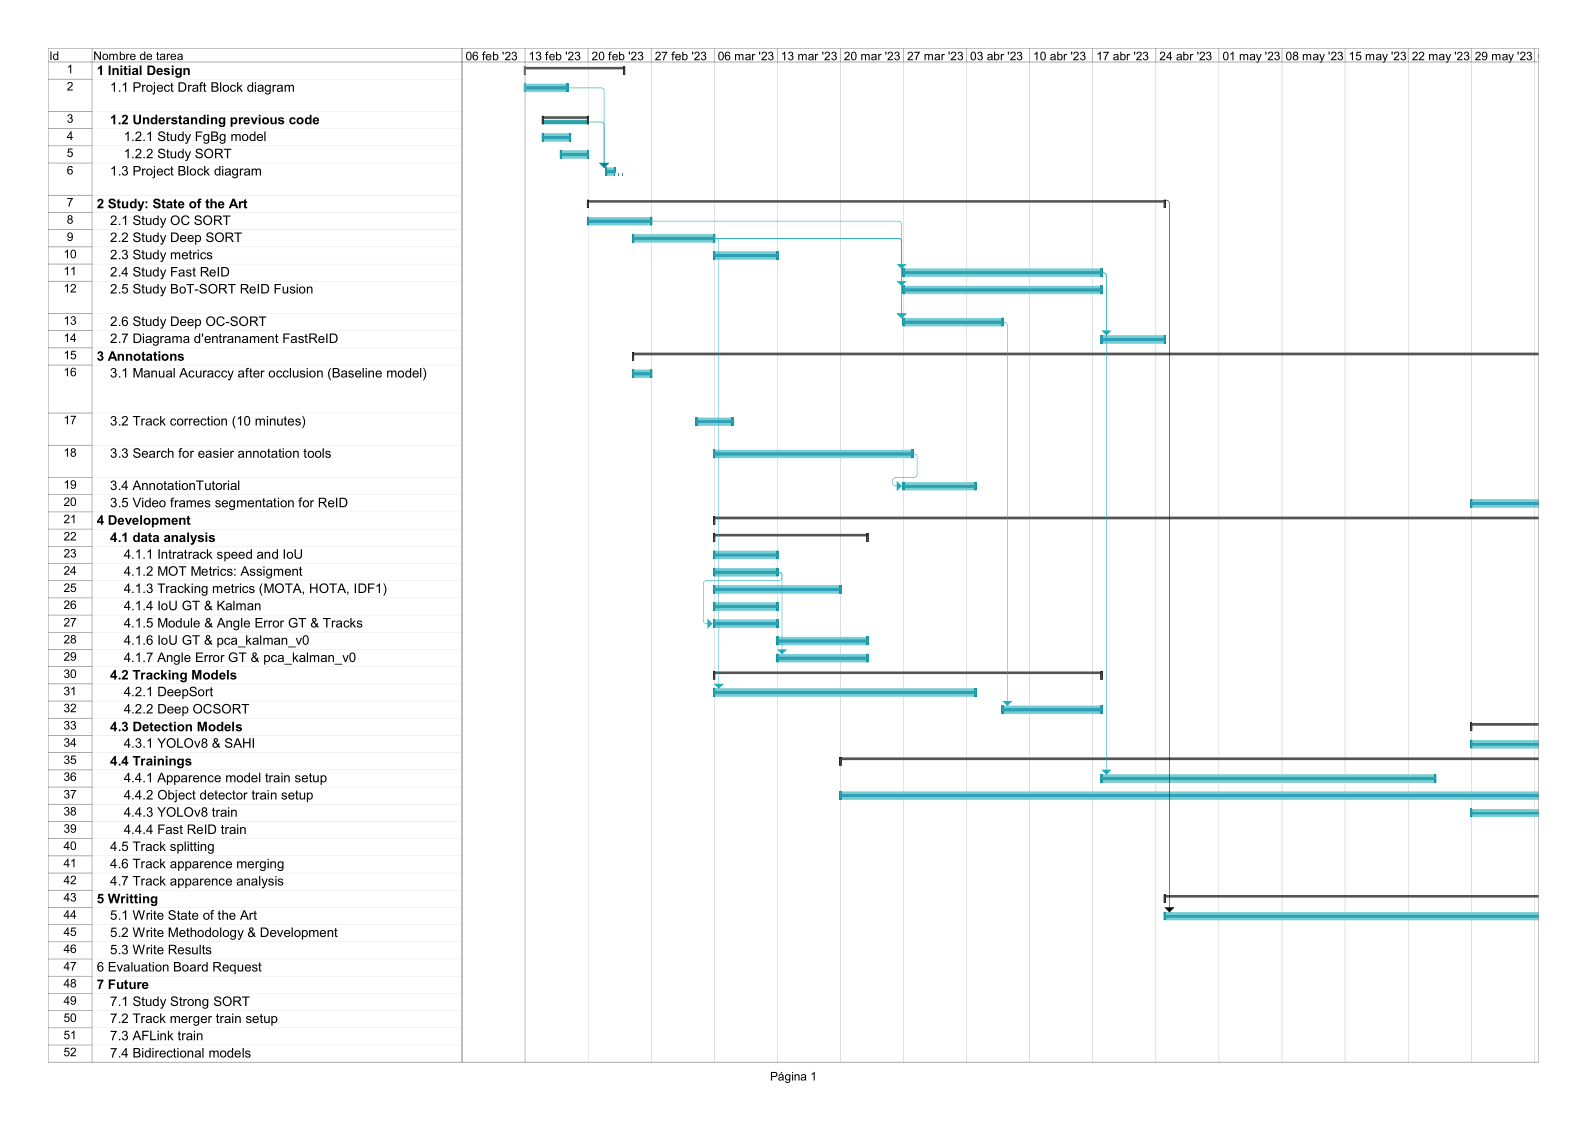
\includegraphics[width=\linewidth]{figures/03_introduction/gantt1.png}
%        \caption[Project's Gantt diagram 2]{\footnotesize{Gantt diagram of the second half of the project}}
%        \label{fig:gantt_2}
%    \end{subfigure}
%    \caption[Project's Gantt diagram]{\footnotesize{Gantt diagram of the project}}
%    \label{fig:gantt}
%\end{figure}
